\documentclass[article]{jss}

\usepackage{orcidlink,thumbpdf,lmodern}
\usepackage{amssymb,amsmath,amsthm,mathtools,bm}
\usepackage{upquote}

\usepackage{microtype}
\UseMicrotypeSet[protrusion]{basicmath} % disable protrusion for tt fonts

\usepackage{booktabs}
\usepackage{caption}
\usepackage{subcaption}
\usepackage{siunitx}

\usepackage[linesnumbered,vlined,ruled]{algorithm2e}

\usepackage{enumitem}

\usepackage{todonotes}

% Workaround for Gin settings
\makeatletter
\let\natwidth\Gin@nat@width
\makeatother

\DeclareMathOperator*{\minimize}{minimize}
\newcommand{\link}{g}
\newcommand{\ilink}{g^{-1}}
% \newcommand{\link}[1]{\expandafter\newcommand\csname #1\endcsname[1]{#1(##1)}}


% setup url command for hyperref
\newcommand{\myurl}[1]{\href{https://#1}{\nolinkurl{#1}}}

\author{
  Johan Larsson~\orcidlink{0000-0002-4029-5945}\\University of Copenhagen
  \And
  Ma\l{}gorzata Bogdan~\orcidlink{0000-0001-6355-8261}\\University of Wroc\l{}aw
  \And
  Krystyna Grzesiak~\orcidlink{0000-0003-2581-7722}\\University of Wroc\l{}aw
  \AND
  Mathurin Massias~\orcidlink{0000-0002-8950-0356}\\Inria, ENS de Lyon, CNRS
  \And
  Jonas Wallin~\orcidlink{0000-0003-0381-6593}\\Lund University
}
\Plainauthor{}

\title{Efficient Solvers for SLOPE in \proglang{R}, \proglang{Python}, \proglang{Julia}, and \proglang{C++}}
\Plaintitle{Efficient Solvers for SLOPE in R, Python, Julia, and C++}
\Shorttitle{Efficient Solvers for SLOPE}

\Abstract{
  \noindent We present a suite of packages in \proglang{R}, \proglang{Python},
  \proglang{Julia}, and \proglang{C++} that efficiently solves
  the Sorted L-One Penalized Estimation (SLOPE) problem.
  The packages features a highly efficient hybrid coordinate descent
  algorithm that fits generalized linear models (GLMs) and supports
  a variety of loss functions, including Gaussian, binomial,
  Poisson, and multinomial logistic regression. Our implementation
  is designed to be fast, memory-efficient, and flexible.
  The packages support a variety of data structures (dense and sparse matrices, as well
  as out-of-memory matrices) and are designed to efficiently fit the
  full SLOPE path as well as handle cross-validation of SLOPE models,
  including the relaxed SLOPE.
  We present examples of how to use the packages and benchmarks that
  demonstrate the performance of the packages on a variety of both
  real and simulated data and show that our packages outperform
  existing implementations of SLOPE in terms of speed.
}

\Keywords{SLOPE, OWL, regularization, generalized linear models, \proglang{R}, \proglang{Python}, \proglang{Julia}, \proglang{C++}}
\Plainkeywords{SLOPE, OWL, regularization, generalized linear models, R, Python, C++}

\Address{
  Johan Larsson\\
  Department of Mathematical Sciences\\
  Faculty of Science\\
  University of Copenhagen\\
  Universitetsparken 5\\
  2100 København Ø, Denmark\\
  E-mail: \email{jolars@posteo.com}\\
  URL: \url{https://jolars.co/}
}

\begin{document}

\section{Introduction}

Sorted L-One Penalized Estimation
(SLOPE)~\citep{bogdan2013,zeng2014,bogdan2015} is a type of regularized
regression that consists of solving the following convex optimization problem:
\begin{equation}
  \label{eq:slope}
  \minimize_{\beta_0 \in \mathbb{R},\beta \in \mathbb{R}^p}
  \Big(
  P(\beta_0,\beta)
  = F(\beta_0, \beta) + \alpha J_{\lambda}(\beta)
  \Big)
\end{equation}
where \(P\) is the primal problem, \(F\) is the loss function, \(\alpha\) a parameter
that controls the strength of regularization, and \(\lambda\) a non-increasing sequence of penalty weights. \(J\) is the
\emph{sorted $\ell_1$ norm}, defined as
\begin{equation}
  % \label{eq:sl1}
  J_{\lambda}(\beta) = \sum_{j=1}^p \lambda_j |\beta_{(j)}|, \quad
  \text{where}\quad |\beta_{(1)}| \geq |\beta_{(2)}| \geq \ldots \geq
  |\beta_{(p)}|,
\end{equation}
and \(\lambda\) is a non-increasing sequence of penalty weights. We will
assume that \(F\) takes the following form:
\[
  F(\beta_0, \beta) = \frac{1}{n} \sum_{i=1}^n f(\beta_0 + x_i^\intercal \beta, y_i),
\]
where \(f\) is a smooth, convex function and \(x_i\) is the \(i\)th row of the
\(n \times p\) design matrix \(X\). Throughout the paper, we will use the
convention of denoting a row of a matrix \(X\) as \(x_i\) and a column as
\(x_j\). \(y_i\) is the \(i\)th row of the \(n \times m\) response matrix
\(Y\),\footnote{For our case, \(m = 1\) unless the model is multinomial
  logistic regression.}
and we let \((\hat{\beta}_0,
\hat{\beta})\) denote a solution to the problem in \autoref{eq:slope}.

SLOPE is a generalization of both the lasso\footnote{The lasso is attained by
  taking a constant
  \(\lambda\).}~~\citep{santosa1986,donoho1994,donoho1995,tibshirani1996} and
OSCAR\footnote{OSCAR is attained by setting \(\lambda\) to be a linear
  sequence, \(\lambda_j = \theta_1 + \theta_2(p - j)\) with \(\theta_1,
  \theta_2 \geq 0\)~\citep{figueiredo2014}.} (octagonal shrinkage and clustering
algorithm for regression)~\citep{bondell2008}.
One of the most important properties of SLOPE is that it can cluster coefficients by
setting them to the same magnitude~\citep{figueiredo2016,bogdan2022}. This is a natural
consequence of the sorted \(\ell_1\) norm, stemming from the fact that
the contribution to the norm of a given coefficient increases disproportionally if it
changes order. This also allows SLOPE to better recover ordering patterns
in the solution.

Like the lasso, SLOPE is a convex but non-smooth optimization problem. And since the
pool-adjacent-violators algorithm~(PAVA)~\citep{barlow1972} can be used to
efficiently\footnote{At an average \(p \log p\) rate, due to the limiting
  sorting operation.} compute the proximal operator of the sorted \(\ell_1\)
norm, it is possible to use a wide range of proximal algorithms, such
as proximal gradient descent, to solve SLOPE. This also includes accelerated
methods such as FISTA~\citep{beck2009}, which was for instance used by
\citet{bogdan2015}. Other possibilities include proximal Newton~\citep{lee2014}
and the alternating direction method of multipliers (ADMM) method~\citep{boyd2010}.

For similar problems such as the lasso and
elastic net\citep{zou2005}, however, these
aforementioned methods have generally found themselves outperformed by coordinate
descent methods~\citep{friedman2007,friedman2010}, which optimize one
coefficient at a time. Unfortunately, coordinate descent requires that the
objective is separable in \((\beta_0, \beta)\), which is not the case in SLOPE
due to the permutations involved in the sorted \(\ell_1\) norm, which means
that coordinate descent cannot be used directly. This problem was, however,
overcome by \citet{larsson2023}, who invented a hybrid combination of proximal
gradient and coordinate descent. The algorithm alternates between proximal gradient
descent steps on the full problem and coordinate descent on a collapsed
problem corresponding to the current cluster structure to achieve
robust and fast convergence.

In this paper we make this algorithm available to a wide audience, by
presenting a collection of packages in \proglang{R}, \proglang{Python},
\proglang{Julia}, and \proglang{C++}.

\subsection{Outline of the paper}

In \autoref{sec:math-details}, we introduce the statistical problem that our
packages solve, namely generalized linear models (GLMs) regularized with the sorted
\(\ell_1\) norm (SLOPE)\footnote{SLOPE is sometimes used only as the procedure
  that uses quadratic loss, but here we adopt a more general terminology and
  let SLOPE be defined for any loss function.}, and provide a brief overview of
the mathematical properties of GLMs and the particular properties of SLOPE.
We discuss the optimization problem and describe the hybrid
coordinate descent algorithm we use for solving SLOPE.
In \autoref{sec:implementation-details}, we provide a detailed overview of the
software implementations, highlighting technical aspects such as
memory management, parallelization, and convergence criteria.
In \autoref{sec:examples}, we showcase how our packages work in practice,
providing examples of fitting models, plotting, and cross-validation.
Finally, in \autoref{sec:discussion}, we summarize the contributions of this paper
and discuss future work.

\section{Mathematical details}\label{sec:math-details}

In this section, we provide a brief overview of the mathematical
details of the SLOPE optimization problem, including the objective and
the hybrid coordinate descent algorithm used to solve it. We also discuss the
convergence criteria used to determine when the algorithm has converged, and
the path fitting procedure used to compute the full regularization path for SLOPE.

\subsection{Generalized linear models}
% \label{sec:glm}

Our packages are designed to solve SLOPE for generalized linear models (GLMs),
in which the loss function is defined as
\[
  F(\beta_0, \beta) = \frac{1}{n} \sum_{i=1}^n f(\eta, y_i),
\]
letting \(\eta_i = x_i^\intercal \beta + \beta_0\) be the linear predictor. The
response \(y_i\) is modelled as a random variable from an exponential family,
and is assumed to depend conditionally on the linear predictor \(\eta_i\)
through \(\E(y_i \mid \eta_i) = \ilink(\eta_i)\), where \(\ilink\) is the
inverse link function.

To estimate the parameters of the model, \((\beta_0, \beta)\), we form a loss
function from the negative log-likelihood of the target distribution, modeling
its mean parameter through the inverse link funktion applied to the linear
predictor. A special property of the resulting loss function is that its partial
derivative with respect to \(\eta\) is the
\emph{generalized residual}
\[
  \frac{\partial}{\partial \eta_i} f(\eta_i, y_i) = \ilink(\eta_i) - y_i = r_i.
\]
As a consequence, the gradient of the loss function with respect to \(\beta\)
can be expressed as
\[
  \frac{\partial}{\partial \beta_j} F(\beta_0,\beta)
  = \frac{1}{n} \sum_{i=1}^n x_{ij} \frac{\partial}{\partial \eta_i} f(\eta_i, y_i)
  = \frac{1}{n} \sum_{i=1}^n x_{ij} r_i.
\]

We summarize the loss functions, link functions, and inverse link functions
for the GLMs supported by the SLOPE packages in \autoref{tab:glm}.

\begin{table}[t!]
  \centering
  \begin{tabular}{lccc}
    \toprule
    Model       & \(f(\eta, y)\)                                                                                       & \(\link(\mu)\)                            & \(\ilink(\eta)\)                                       \\
    \midrule
    Gaussian    & \(\frac{1}{2}(y - \eta)^2\)                                                                          & \(\mu\)                                   & \(\eta\)                                               \\
    \addlinespace
    Binomial    & \(\log(1 + e^\eta) - \eta y\)                                                                        & \(\log \left(\frac{\mu}{1 - \mu}\right)\) & \(\frac{e^\eta}{1 + e^\eta}\)                          \\
    \addlinespace
    Poisson     & \(e^\eta - \eta y\)                                                                                  & \(\log(\mu)\)                             & \(e^\eta\)                                             \\
    \addlinespace
    Multinomial & \(\sum_{k=1}^{m-1}\left( \log \left( 1 +  \sum_{j=1}^{m-1} e^{\eta_j}\right) - y_k \eta_k  \right)\) & \(\log\left(\frac{\mu}{1 - \mu}\right) \) & \(\frac{\exp(\eta)}{1 + \sum_{j=1}^{m-1} e^{\eta_j}}\) \\
    \bottomrule
  \end{tabular}
  \caption{Loss functions, link functions, and inverse link functions for
    generalized linear models in the SLOPE package. Note that in the case of
    multinomial logistic regression, the input is vector-valued, and we allow
    \(\log\) and \(\exp\) to be overloaded to apply element-wise in these cases.
  }
  \label{tab:glm}
\end{table}

A particular case of interest is the multinomial logistic regression model.
Many implementations of regularized multinomial logistic regression models, such
as those by \citet{friedman2010} and \citet{fercoq2015} use the \emph{redundant}
\(m\)-class formulation. Here, however, we have opted to use the non-redundant
formulation of the loss function, with the last class serving as the reference
category. This choice complicates notation slightly and leads to a more
complex formulation for the dual problem. For SLOPE, however, this is a
more natural choice since it generalizes to the binary case as well (in which
the last class is also implicit).\footnote{SLOPE needs a \(\lambda\) sequence of length
  \(mp\), so the loss function for the multinomial case would not be equivalent
  to the binary case if we used the redundant formulation.} Furthermore, it also
relieves the problem of the parameter ambiguity that affects the redundant
formulation, where rows of the coefficient matrix can be shifted
without changing the value of \(F(\beta_0, \beta)\). This also means that
the redundant formulation needs to be accompanied by a bounds adjustment step~\citep{friedman2010}.
This is trivial in the case of the lasso and ridge and
only slightly more complicated in the case of elastic net. For SLOPE, however,
the situation is much more involved since rows of the coefficient matrix cannot
be arbitrarily shifted, since this might affect the entire clustering
structure.

\subsection{Hybrid algorithm}

The primary algorithm of the \pkg{SLOPE} packages is the hybrid coordinate
descent algorithm by \citet{larsson2023}. Since it is described in detail
there, we will only summarize its key points here and highlight
some of the improvements that we have made to the original algorithm.
The basic idea is to perform the coordinate descent updates on
the clusters' coefficients rather than directly on the coefficients. In principle,
we fix the current cluster and update all coefficients belong to it in a single step.
On its own, this algorithm is not guaranteed to converge since it can only
reorder or merge clusters. In order to circumvent this, the algorithm must
therefore be combined with proximal gradient descent steps. These steps
are able to split the clusters, which eventually means that the full
algorithm converges to the correct clusters and global minimum.

We have outlined the algorithm in \autoref{alg:hybrid}. Unlike the implementation
in \citet{larsson2023}, this algorithm is extended to
any generalized linear model---not just the Gaussian case. To do so,
we use a iteratively reweighted least-squares (IRLS) approach, determining
weights \(w\) and a working response \(z\) after each proximal gradient descent step.
We then run the coordinate descent algorithm for a fixed number of iterations.
Convergence is monitored using a duality-based stopping criterion~(\autoref{sec:convergence-criteria-details}), which
we check after each gradient is computed. In order to avoid complicating
the presentation, we have omitted some details of the algorithm here.

\begin{algorithm}[tp]
  \caption{
    The Hybrid coordinate descent algorithm for generalized linear models, using
    the IRLS where weights \(w\) and a working response \(z\) are computed
    after a proximal gradient descent step. We describe the cyclical version of
    the algorithm here. \(c^{\setminus k}\) is a version of the vector \(c\)
    with the \(k\)th coefficient omitted and \(T\) is the SLOPE thresholding
    operator, which we have illustrated in \autoref{fig:slope-thresholding}.
  }
  \label{alg:hybrid}
  \SetKwInOut{Input}{input}
  \SetKwComment{tcc}{$\triangleright$ }{}
  \SetCommentSty{textit}

  \Input{%
    \(X \in \mathbb{R}^{n\times p}\),
    \(y\in \mathbb{R}^n\),
    \(\lambda \in \{\mathbb{R}^p : \lambda_1 \geq \lambda_2 \geq \cdots > 0\}\),
    \(v \in \mathbb{N}\)
  }

  \Repeat{\(P(\beta_0, \beta) - D(\theta) \leq \varepsilon|P(\beta_0, \beta)|\)}{

    Set \(t\) with backtracking line search\;

    \(\beta \gets \beta - t \nabla F(\beta_0, \beta)\)\;

    \For{\(i \gets 1,\dots,n\)}{

      \(\eta_i \gets x_i^T \beta + \beta_0 \)\;
      \(w_i \gets \frac{\partial}{\partial \eta_i} f(\eta_i, y_i) \)\tcc*{Weights for IRLS}
      \(z_i \gets \eta_i - \frac{r_i(\eta_i, y_i)}{w_i} \)\tcc*{Working response for IRLS}
    }
    Update \(c\), \(\mathcal{C}\)\;
    \For{\texttt{it} \(\gets 1,\dots,\)\texttt{cd\_maxit}}{
      \(k \gets 1\)\;
      \(\beta^\text{old} \gets \beta\)\;

      \While{\(k \leq \lvert \mathcal{C} \rvert\)}{
        \(\tilde x \gets \sum_{j \in \cC_k} x_j \sign \beta_j \)\;
        \(\tilde{r} \gets X \beta + \beta_0 - z\)\tcc*{Residuals}
        \(\gamma \gets \frac{1}{n} \sum_{i=1}^n w_i \tilde{x}_i \tilde{r}_i\)\tcc*{Gradient}
        \(\xi \gets \frac{1}{n} \sum_{i=1}^n w_i \tilde{x}_i^2 \)\tcc*{Hessian}
        \(\tilde {c} \gets T(c_k \xi - \gamma; \xi, c^{\setminus k}, \lambda)\)\;
        \(\beta_{\cC_k} \gets \tilde{c} \sign(\beta_{\cC_k})\)\;
        Update \(c\), \(\mathcal{C}\)\;
        \(k \gets k + 1\)\;
      }

      \If{\(P(\beta) \geq P(\beta^\text{old})\)}{
        \(\beta \gets \beta^\text{old}\)\;
        break\;
      }
    }
  }

\end{algorithm}

\begin{figure}[t]
  \centering
  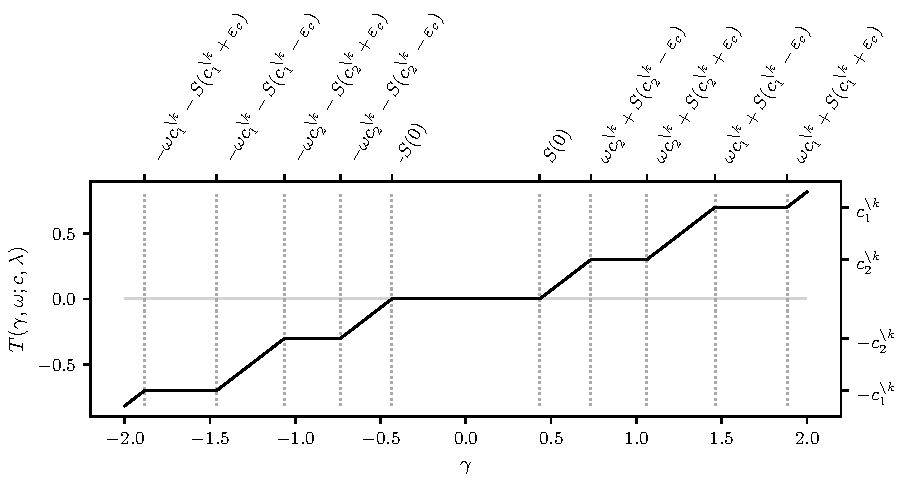
\includegraphics[width=\natwidth]{images/slope-thresholding.pdf}
  \caption{
  An illustration of the SLOPE thresholding operator for \(\beta = [0.5, -0.5, 0.3, 0.7]^\intercal\),
  so that \(c = (0.7, 0.5, 0.3)\) and consequently \(c^{\setminus k} = (0.5, 0.3)\).
  The example and figure are adapted from \citet{larsson2023}.
  In the example, we are considering an update for the second cluster (\(k = 2\)).
  Define \(S(x) = \sum_{j \in
    C(x)}\lambda_{(j)^-_{x}}\) and let \(\varepsilon_c > 0\) be defined such that
  \(\varepsilon_c < \big| c_i - c_j\big|\;\forall\, i \neq j\) and
  \(\varepsilon_c < c_m\) if \(c_m \neq 0\).
  . Across regions where the function is constant,
  the operator sets the result to be either exactly 0 or to the value of one
  of the elements of \(\pm c^{\setminus k}\).
  }
  \label{fig:slope-thresholding}
\end{figure}

The hybrid nature of the algorithm is not only useful for enabling the
coordinate descent steps, but also comes with benefits due to the inclusion of
the PGD steps. Proximal gradient descent algorithms are known to converge under
more general assumptions than coordinate descent algorithms~\citep{wright2015},
which means that the PGD part of the algorithm can serve as a fallback in case
the coordinate descent part does not converge. In practice, we store the
current solution before updating and revert to it if the coordinate descent
step does not improve the primal objective.

The implementation in \citet{larsson2023} used a type of cyclical coordinate
descent in which the algorithm iterated over the clusters in descending order
by their coefficients' magnitudes. Although simple to implement
and efficient for many problems, cyclical coordinate descent is known
to suffer from convergence issues in some cases~\citep{wright2015}, which
we found to be the case for SLOPE as well.
For the current implementation, we therefore include as well as default
to a version using random permutations, which is slightly slower but
more robust.

\subsection{Convergence criteria}

Our packages use a duality-based stopping criterion, providing an upper bound
on suboptimality at convergence. We transform the primal problem into a
constrained formulation and derive a dual problem that allows us to compute a
duality gap. As a stopping criterion, we use the relative duality gap: \[
  P(\beta_0, \beta) - D(\delta) \leq \varepsilon | P(\beta_0, \beta) |, \] where
\(\varepsilon >0\) is the user-defined tolerance level. This provides a
reliable, solver-independent measure of convergence. The complete derivation of
the dual problem and the calculation of the duality gap is provided in
\autoref{sec:convergence-criteria-details}.

\subsection{Path fitting}
% \label{sec:path-fitting}

Since optimal settings of \(\alpha\) are only available under strict
assumptions that are typically hard to test, it is common to instead use
cross-validation to tune \(\alpha\) over a grid of values. In practice, this
means that we repeatedly have to fit the full regularization path, which is the
sequence of solutions to the problem in \autoref{eq:slope} as \(\alpha\) is varied
from \(\alpha_\text{max}\), at which point the first cluster enters the model,
to a small value of \(\alpha\) at which the model is almost saturated. Our
packages are optimized to efficiently compute the full regularization path, and
make use of  screening rules~(\autoref{sec:screening-rules}) to speed up the
process of doing so.

We use the same criteria as \citet{friedman2010} for stopping the path early,
except that we stop if the number of \emph{clusters} excluding the zero-cluster
exceeds \(n + 1\) (by default), since the support of SLOPE is limited at \(n\)
clusters\footnote{ As opposed to the lasso, which at most allows \(n\) non-zero
  \emph{coefficients}. }, which can potentially exceed the number of non-zero
coefficients.\footnote{In practice this is quite rare since clusters do not
  form easily at low levels of regularization.}

\subsection{Screening rules}\label{sec:screening-rules}

Sparse models like lasso and SLOPE are well-known to benefit from
\emph{screening rules}, which are used to reduce the dimension of \(\beta\) in
the optimization problem and thereby speed up optimization. The intuition for
this is that it is possible to estimate the gradient \(\nabla F(\beta) \) for a
given SLOPE problem and, via the subdifferential, estimate the support of the
solution: the identity of the nonzero coefficients. Screening rules are
either \emph{heuristic} or \emph{safe}. In the latter case the rule guarantees that
excluded predictors correspond to zero coefficients in the final model. Heuristic
rules, on the other hand, do not guarantee this and therefore need to be
complemented with a pass over all coefficients at the end to ensure that the
optimality conditions are satisfied. Since they are less conservative, however,
the cost of doing so may be outweighed by the savings in computation
time.

In the SLOPE package, we use the strong screening rule for
SLOPE~\citep{larsson2020a}, which is an extension of the working set strategy
for the strong screening rule for the lasso~\citep{tibshirani2012}.

\section{Implementation details}
\label{sec:implementation-details}

In this section, we provide a detailed overview of the implementation
details of the SLOPE packages, including the data structures used to represent
the clusters, the thresholding operator, and parallelization strategies.

\subsection{Software architecture}
% \label{sec:software}

We have implemented a collection of packages for solving SLOPE, currently with
support for \proglang{R}, \proglang{Python}, and \proglang{Julia}. The backbone
of all of these packages is based on a \proglang{C++} library that implements
all of the numerical algorithms for SLOPE, including preprocessing,
cross-validation, and path fitting. The packages for the high-level languages
all serve as thin wrappers to the \proglang{C++} library, with some additional
functionality for handling data and plotting the results. This means that new
features and bug fixes propagate quickly and easily to all these wrapppers and
enable users to promptly take advantage of the latest developments. The entire
suite of packages is open source and available in version-controlled
online repositories~(\autoref{tab:slope-packages}).

\begin{table}[tp]
  \centering
  \begin{tabular}{llll}
    \toprule
    Language          & Package        & Repository                         & Documentation                     \\
    \midrule
    \proglang{R}      & \pkg{SLOPE}    & \myurl{github.com/jolars/SLOPE}    & \myurl{jolars.github.io/SLOPE}    \\
    \proglang{Python} & \pkg{sortedl1} & \myurl{github.com/jolars/sortedl1} & \myurl{jolars.github.io/sortedl1} \\
    \proglang{Julia}  & \pkg{SLOPE.jl} & \myurl{github.com/jolars/SLOPE.jl} & \myurl{jolars.github.io/SLOPE.jl} \\
    \proglang{C++}    & \pkg{slope}    & \myurl{github.com/jolars/libslope} & \myurl{jolars.github.io/libslope} \\
    \bottomrule
  \end{tabular}
  \caption{A summary of the suite of packages that we have developed for solving SLOPE, along
    with links to the source code repositories and documentation.}
  \label{tab:slope-packages}
\end{table}

This is made possible via several pieces of software that enable us to link the
API from our \proglang{C++} library to the high-level languages. This includes
\pkg{Rcpp}~\citep{eddelbuettel2011} and \pkg{RcppEigen}~\citep{bates2013} for
\proglang{R}, \pkg{pybind11}~\citep{jakob2025}, and \pkg{CxxWrap}~\citep{janssens2020} for
\proglang{Julia}.

\subsection{Core algorithmic components}

Handling the cluster structure of SLOPE is a key part of the algorithm since we
will both be iterating over the clusters as part of the coordinate descent
updates as well as updating the clusters after each update. In our
implementation, we represent the clusters as a collection of three vectors:

\begin{description}
  \item[\code{c}] The coefficients of the clusters
  \item[\code{c\_idx}] Pointers to the coefficients in the cluster
  \item[\code{c\_ptr}] Values of the cluster pointers
\end{description}

In this representation, the indices for the \(k\)th cluster are given by \code{
c_idx[c_ptr[k] : c_ptr[k+1]]} and the coefficient is simply \code{c[k]}.
This structure is the same basic setup as in \citet{larsson2023}. Unlike
their implementation, however, we have made improvements to the
handling of updating the clusters (merging,
reordering, removal), which can now be performed with negligible
overhead and with minimal copying.

The SLOPE thresholding operator~(\autoref{fig:slope-thresholding}) is the analogue
to the soft-thresholding operator for the lasso. But unlike the latter, which
is trivial to compute, the SLOPE thresholding operator needs to conduct a
search over the clusters in order to find correct solution. This leads to a
worst-case complexity that depends on the number of clusters, which might seem
to be prohibitive when both \(n\) and \(p\) are large. Fortunately, however,
the situation is much less dire in practice, since the order of the clusters
typically stabilizes early during optimization. This also means that, contrary
to conventional wisdom, it is in fact more efficient to conduct a linear, as opposed
to binary, search over the clusters. Note also that the partial \(\lambda\) sums
do not need to be computed directly. Instead, we simply compute the
cumulative sum of the \(\lambda\) array once and use this to retrieve
the partial sums as needed.

\subsection{Data handling and optimization}

Our package is based on the \pkg{Eigen} \proglang{C++} library and provides
support for both dense and sparse design matrices. The latter can be
constructed through the \pkg{Matrix}~(\proglang{R}),
\pkg{scipy}~(\proglang{Python}), and \pkg{SparseArrays}~(\proglang{Julia})
packages in and are passed to the \proglang{C++} API without copying
and with negligible overhead. Coefficients are returned in a sparse format, which
allows for efficient storage and retrieval of the coefficients.

For dense matrices, the packages implement memory-efficient views of the input
matrices in order to avoid copies of the data. This means, for instance, that
no copies need to be made when separating data sets into training and test
data. Due to this memory-efficient implementation, we provide an option to
altogether avoid copying the data during cross-validation. This allows us to
parallelize the cross-validation procedure over arbitrarily many folds and
repetitions without needing to ever copy the data, which makes for a much
much more memory-friendly implementation (at the cost of
worse runtime performance).

The SLOPE packages also support out-of-memory storage for the design matrix, which
means that users can fit SLOPE models on data sets that are larger than the
available memory. Storage in RAM is therefore limited to the order of \(O(n) +
O(p)\), which means that the packages can be used on huge data sets.
This is supported via the generic \code{Eigen::Map} class, which allows
arbitrary data to be mapped into \pkg{Eigen} data structures. At the
time of writing, this is only supported for \proglang{R},
which is possible via the \pkg{bigmemory} package~\citep{kane2013},
and currently only for dense designs.

As shown by \citet{larsson2025}, predictor normalization (centering and
scaling the design matrix) may have large consequences for the
solutions. In our packages, we provide multiple different options
for centering and scaling, independently of one another.
We also provide the possibility to manually supply centering
and scaling vectors. Optionally, normalization is also realized just-in-time (JIT),
which means that the design matrix does not need to be normalized in place.
Normalization is performed as predictors of the design matrix are accessed during
optimization, which allows us to support centering even of sparse design
matrices. This also allows us to completely avoid copying the design matrix.

The software is parallelized using \pkg{OpenMP}, which is supported on all
major platforms. Our functions employ several heuristics based on problem size to
determine whether to spawn multiple threads, except
for the case of cross-validation, which is always parallelized.

\section{Examples}\label{sec:examples}

The packages are
available through the respective package managers for each language, and can be
be installed using the following commands:
\begin{description}[labelwidth=8ex]
  \item[\proglang{R}] \code{R> install.packages("SLOPE")}
  \item[\proglang{Python}] \code{$ pip install sortedl1}
  \item[\proglang{Julia}] \code{julia> using Pkg; Pkg.add("SLOPE")}
\end{description}

Installing the \proglang{C++} library is slightly more involved, and requires
\pkg{CMake}~\citep{kitware2025} together with a working \proglang{C++} toolchain, including
the \pkg{Eigen} library~\citep{guennebaud2010a} and \pkg{OpenMP}~\citep{dagum1998} (optionally,
to enable parallelization).

Assuming that we have loaded a data set consisting of a design
matrix \code{x} and response vector \code{y}, we can fit the full regularization
path for the SLOPE model using the following commands for the different languages:

\begin{minipage}[t]{0.24\textwidth}%
  \textbf{\proglang{R}}
  \begin{Code}
R> library(SLOPE)
R> fit <- SLOPE(x, y)
  \end{Code}
\end{minipage}
\hfill
\begin{minipage}[t]{0.33\textwidth}%
  \textbf{\proglang{Python}}
  \begin{Code}
>>> import sortedl1
>>> model = sortedl1.Slope()
>>> fit = model.path(x, y)
  \end{Code}
\end{minipage}
\hfill
\begin{minipage}[t]{0.32\textwidth}%
  \textbf{\proglang{Julia}}
  \begin{Code}
julia> using SLOPE
julia> fit = slope(x, y)
  \end{Code}
\end{minipage}

\medskip

You can also use the C++ library directly, in
which case the above would translate into the
following:
\begin{Code}
#include <slope/slope.h>
slope::Slope model;
auto path_result = model.path(x, y);
\end{Code}

In the sequel, we will focus our examples on the \proglang{R} package, but
note that all of the functionality we cover is available throughout
the suite of packages and feature similar APIs.

\subsection{First steps}

We start with a simple example of fitting a full SLOPE path to the diabetes
data set~\citep{efron2004}, including plotting it.\footnote{Note that
  the actual for the plotting examples here is slightly more complex
  to allow for better control over the aesthetics.}

\begin{Code}
R> library(SLOPE)
R> data("diabetes", package = "lars")
R> x <- scale(diabetes$x)
R> y <- diabetes$y
R> fit_slope <- SLOPE(x, y, q = 0.1)
R> plot(fit_slope)
\end{Code}

The \code{q} parameter is a parameter of the sequence of \(\lambda\) values,
which by default~(\code{lambda = "bh"}) is the Benjamini--Hochberg (BH)
sequence~\citep{bogdan2015}. If the design matrix is orthogonal, then the
\code{q} parameter sets a desired false discovery rate (FDR) in terms
of the identification of true signals (nonzero coefficients).

Other types of sequences are also supported,
including \code{lambda = "lasso"} for the lasso
\code{lambda = "oscar"} for the OSCAR sequence~\citep{bondell2008}, and
\code{lambda = "gaussian"} for the Gaussian-type sequence~\citep{bogdan2015},
which is a modification of the BH sequence that has been empirically shown to
provide similar FDR control in non-orthogonal, low-dimensional settings.

To show how the choice of the \(\lambda\) sequence affects the
results, we will refit the diabetes data using the lasso sequence.

\begin{Code}
R> fit_lasso <- SLOPE(x, y, lambda = "lasso")
R> plot(fit_lasso)
\end{Code}

The resulting paths are plotted in \autoref{fig:diabetes}. Observe that the
paths are overall similar but that the SLOPE path has clustered
some coefficients for parts of the path. Predictors 3 and 9, for instance,
enter the path together and remain clustered at the beginning, then
split apart and again cluster together briefly, before diverging again.
We also see that predictor 6 joins the path briefly together
with predictor 5 on the SLOPE path, but then return to zero until
it later enters again on its own.

\begin{figure}[tp]
  \centering
  {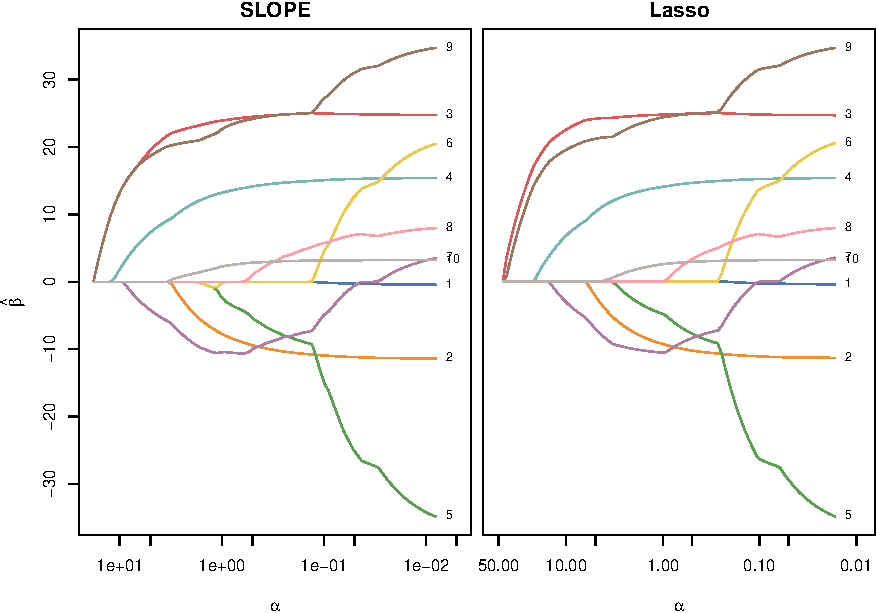
\includegraphics[width=\natwidth]{images/diabetes-slope-lasso.pdf}}
  \caption{%
    SLOPE and lasso paths on the diabetes
    data set. Note that the \(x\) axis is reversed. Numbers indicate
    the indices of the predictors.
  }
  \label{fig:diabetes}
\end{figure}

% TODO: We first need to implement this in the package.

\subsection{Relaxed SLOPE}

To attain sparsity, SLOPE shrinks coefficients towards zero. This introduces
bias, which, although it helps to combat overfitting, may also lead to
worse predictions in some cases. To mitigate this, it is possible
to \emph{relax} the SLOPE solutions by fitting an ordinary least-squares
model to the collapsed cluster structure from running SLOPE~\citep{skalski2022}\footnote{
  Note that this paper refers to the relaxed SLOPE as the \emph{debiased} SLOPE. Here,
  we prefer the term relaxed to stay closer to the nomenclature from the lasso literature and
  avoid confusion with the debiased lasso~\citep{geer2014}, which represents a different approach.}.
The level of relaxation is parameterized by \(\gamma\), which controls the mix between the
original SLOPE solution (\(\gamma = 1\) and the fully relaxed
solution (\(\gamma = 0\)), so that
the end result is given by
\[
  \hat{\beta} = \gamma \hat{\beta}_\text{SLOPE} + (1 - \gamma) \hat{\beta}_\text{relaxed}.
\]

Our packages support regularization through the \code{gamma} argument.
Here, we fit two models, one that is fully relaxed
(\(\gamma = 0\)) and one that is semi-relaxed (\(\gamma = 0.5\)).

\begin{Code}
R> fit_relaxed <- SLOPE(x, y, q = 0.1, gamma = 0)
R> fit_semirelaxed <- SLOPE(x, y, q = 0.1, gamma = 0.5)
\end{Code}

We plot the resulting paths in \autoref{fig:relaxed-slope}. Observe
the jaggedness of the relaxed paths, which change dramatically
as clusters form, merge, and split.

\begin{figure}[tp]
  \centering
  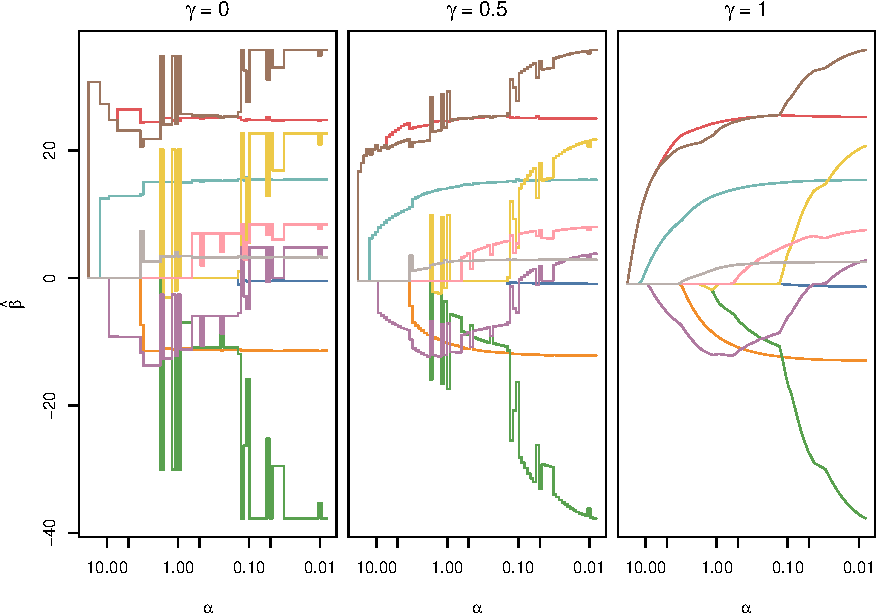
\includegraphics[width=\natwidth]{images/slope-relaxed.pdf}
  \caption{%
    SLOPE with various level of relaxation \(\gamma\), with
    \(\gamma = 0\) (fully relaxed), \(\gamma = 0.5\) (semi-relaxed),
    and \(\gamma = 1\) (standard SLOPE).
  }
  \label{fig:relaxed-slope}
\end{figure}

\subsection{Cross-validation}

Our packages support hyper-parameter tuning via iterated \(k\)-fold
cross-validation (CV), with parameterization over \(\alpha\), \(\lambda\) type (BH,
Gaussian type, etc.), \(\gamma\) (SLOPE relaxation parameter).
Here, we demonstrate the CV functionality by cross-validating across
to values of the \(q\) parameter and printing the results,
which displays the optimal values for all the cross-validated parameters.

\begin{CodeChunk}
  \begin{CodeInput}
R> set.seed(48)
R> fit_cv <- cvSLOPE(x, y, q = c(0.1, 0.2))
R> fit_cv
\end{CodeInput}
  \begin{CodeOutput}
Call:
cvSLOPE(x = x, y = y, q = c(0.1, 0.2))

Optimum values:
      q gamma     alpha measure     mean       se      lo       hi
129 0.2     0 0.3379402     mse 3013.065 234.6321 2482.29 3543.839
\end{CodeOutput}
\end{CodeChunk}

It also easy to plot the cross-validation results~\autoref{fig:cv}, which
show the cross-validation error with 95\% confidence intervals and
a dashed line indicating the optimal value of \(\alpha\) for the
best value of \(q\).

\begin{Code}
R> plot(fit_cv)
\end{Code}

\begin{figure}[tp]
  \centering
  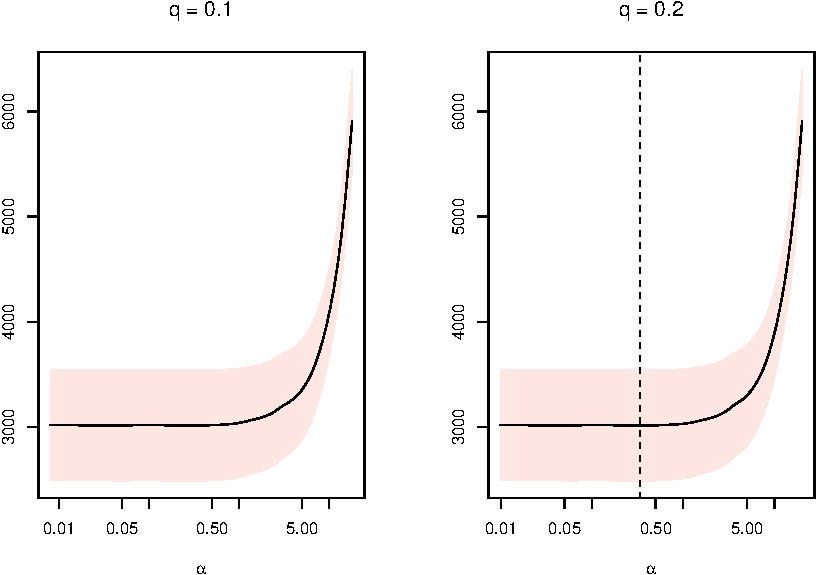
\includegraphics[width=\natwidth]{images/slope-cv.pdf}
  \caption{%
    Mean-squared error (MSE) from cross-validation of
    \(q\) and \(\alpha\) for SLOPE fit to the diabetes data set.
    The dashed line marks the optimal value of \(\alpha\) in the
    panel corresponding to the optimal value of \(q\).
  }
  \label{fig:cv}
\end{figure}

\section{Benchmarks}

In this section, we present benchmarks of the numerical performance of our
implementation for solving SLOPE. In \autoref{sec:single-solution-benchmark}, we examine the performance of SLOPE
when fitting for a single value of \(\alpha\), while in
\autoref{sec:path-benchmark}, we benchmark the performance of fitting
the full regularization path.

Our benchmarks are organized and run using \pkg{benchopt}~\citep{moreau2022a}.
They are available as public git repositories at
\myurl{github.com/benchopt/benchmark\_slope} and
\myurl{github.com/benchopt/benchmark\_slope\_path} for the single solution and
path benchmarks, respectively. Both feature the Python version of our
implementation, \pkg{sortedl1}\footnote{The \proglang{R} package \pkg{SLOPE} is
  also included, but we have omitted it from the benchmark here since it is
  essentially equivalent to the \proglang{Python} package \pkg{sortedl1}.}. The
single solution benchmark includes four variations on proximal gradient
descent (PGD), using Anderson acceleration~\citep{anderson1965,zhang2020},
Barzilai--Borwein step sizes, safe screening rules, and the fast iterative
shrinking and thresholding algorithm (FISTA)~\citep{beck2009}. The latter of
these is also included through the \pkg{skglm} package~\citep{bertrand2022}.
We also include the alternating direction method of multipliers
(ADMM)~\citep{boyd2010}, a semi-smooth Newton-based method~\citep{luo2019},
and an approximate homotopy method, \pkg{SolutionPath}~\citet{dupuis2024},
See \autoref{sec:solver-details} for more details on the solvers and their
implementations. The path benchmark includes a subset of these solvers,
namely \pkg{FISTA}, \pkg{SolutionPath}, and \pkg{ADMM}.

For this paper, we have also created a separate benchmark for fitting the full
regularization path, which is available at
\myurl{github.com/benchopt/benchmark\_slope\_path} and which features a subset
of the solvers from the previous benchmark.

We have run the benchmarks for both simulated~(\autoref{tab:simulated-data}) as
well as real data~(\autoref{tab:real-data}). For all real data, we standardize the
predictors to have mean zero and unit variance if \(X\) is dense and scale with
the maximum absolute value of each predictor otherwise. For all data we use the
Benjamini--Hochberg sequence for \(\lambda\) with \(q=0.2\). Since some of the
solvers cannot handle intercepts, we have omitted the intercepts from the
models. Also note that not all solvers support sparse design matrices, which is
why they are not included everywhere.

\begin{table}[tp]
  \centering
  \begin{tabular}{
      l
      S[table-format=5.0]
      S[table-format=7.0]
      S[table-format=1.5,round-mode=figures,round-precision=2]
      p{5cm}
    }
    \toprule
    Dataset                    & {\(n\)} & {\(p\)} & {\(X\) density} & {References}                        \\
    \midrule
    \dataset{BRCA1}            & 536     & 17322   & 1               & \citet{nationalcancerinstitute2022} \\
    \dataset{Koussounadis2014} & 101     & 34694   & 1               & \citet{koussounadis2014}            \\
    \dataset{Real-Sim}         & 72309   & 20958   & 1               & \citet{mccallum2010}                \\
    \dataset{RCV1}             & 20242   & 44504   & 0.00166         & \citet{lewis2004}                   \\
    \dataset{Rhee2006}         & 842     & 360     & 0.02469         & \citet{rhee2006}                    \\
    \dataset{Scheetz2006}      & 120     & 18975   & 1               & \citet{scheetz2006}                 \\
    \bottomrule
  \end{tabular}
  \caption{%
    List of real datasets used in our experiments, along with some of
    their properties, including the number of samples \(n\) and predictors \(p\).
    \dataset{BRCA1}, \dataset{Koussounadis2014}, and \dataset{Scheetz2006} were
    obtained from \citet{breheny2022} and the rest from \citet{chang2016}.
  }
  \label{tab:real-data}
\end{table}

\begin{table}[tp]
  \centering
  \begin{tabular}{
      l
      S[table-format=6.0]
      S[table-format=6.0]
      S[table-format=2.0]
      S[table-format=1.3]
      S[table-format=0.1]
    }
    \toprule
    {Scenario}       & {\(n\)} & {\(p\)} & {\(k\)} & {\(X\) density} & {\(\rho\)} \\
    \midrule
    High Dim         & 200     & 20000   & 20      & 1               & 0.6        \\
    High Dim, Sparse & 200     & 200000  & 20      & 0.001           & 0.6        \\
    Low Dim          & 200000  & 200     & 40      & 1               & 0.2        \\
    \bottomrule
  \end{tabular}
  \caption{
    Scenarios for the simulated data in our benchmarks. \(\rho\) is the auto-correlation
    between adjacent predictors, \(k\) is the number of clusters, and
    \(n\) and \(p\) are the number of samples and predictors, respectively.
  }
  \label{tab:simulated-data}
\end{table}

\subsection{Single solution}\label{sec:single-solution-benchmark}

We have parameterized our single-solution benchmarks by \(\alpha\) as a
fraction of \(\alpha_\text{max}\) (the value at which the first cluster enters
the model), and run the benchmarks for \(\alpha = \alpha_\text{max}/2\),
\(\alpha_\text{max}/10\), and \(\alpha_\text{max}/50\). We present convergence using
the duality gap.

The results for the simulated data are presented in \autoref{fig:simulated-data-single}.
We can observe that our algorithm is fastest in every case except
the (\(\alpha_\text{max}/50\), High Dim) combination, where the Newt-ALM
method seems to perform better (although does not quite converge). The difference
is especially pronounced for high levels of regularization, where our method is
often many times faster than the next best method.

\begin{figure}[tp]
  \centering
  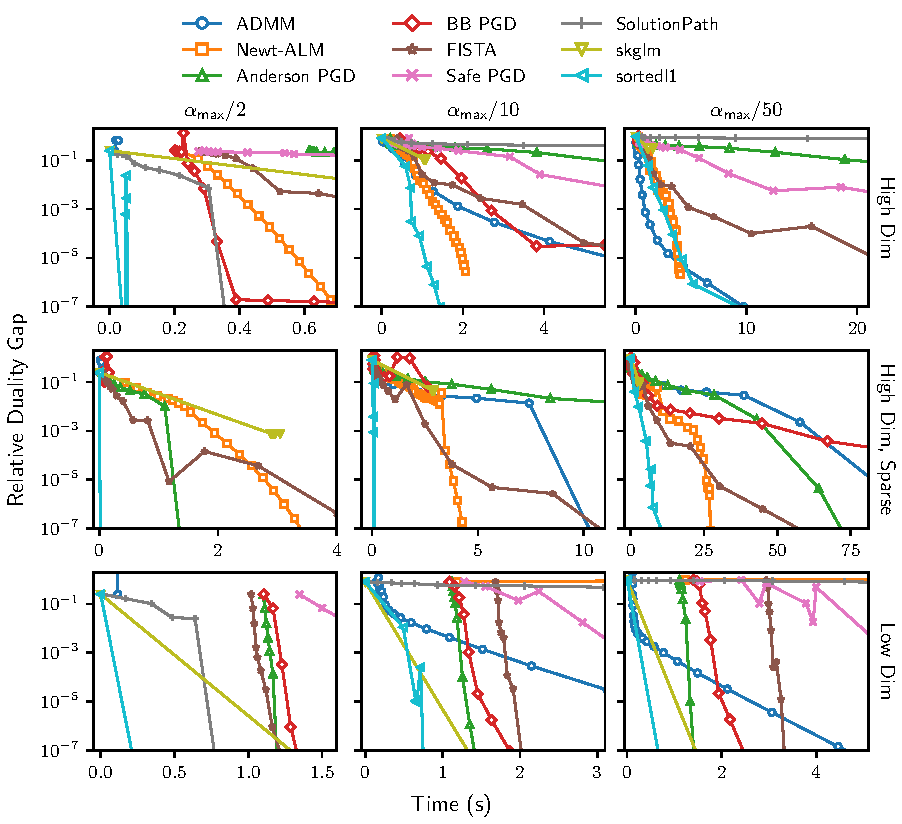
\includegraphics[width=\natwidth]{images/benchmark_single_simulated.pdf}
  \caption{%
    Performance of the solvers for the single solution benchmark for three different settings
    of simulated data~(\autoref{tab:simulated-data}).
    Please see the text for information about the data and setup of the experiment.
  }
  \label{fig:simulated-data-single}
\end{figure}

For real data~\autoref{fig:real-data-single}, we see a mostly similar pattern.
Our algorithm (sortedl1) performs best for most combinations---again dominating
in the high-regularization regime, whereas Newt-ALM and occasionally some version of
the accelerated PGD methods or ADMM perform well. Notice, however, that the other algorithms
performance appears to be much more sensitive to the problem, especially the
ADMM method, which sometimes diverges.

\begin{figure}[tp]
  \centering
  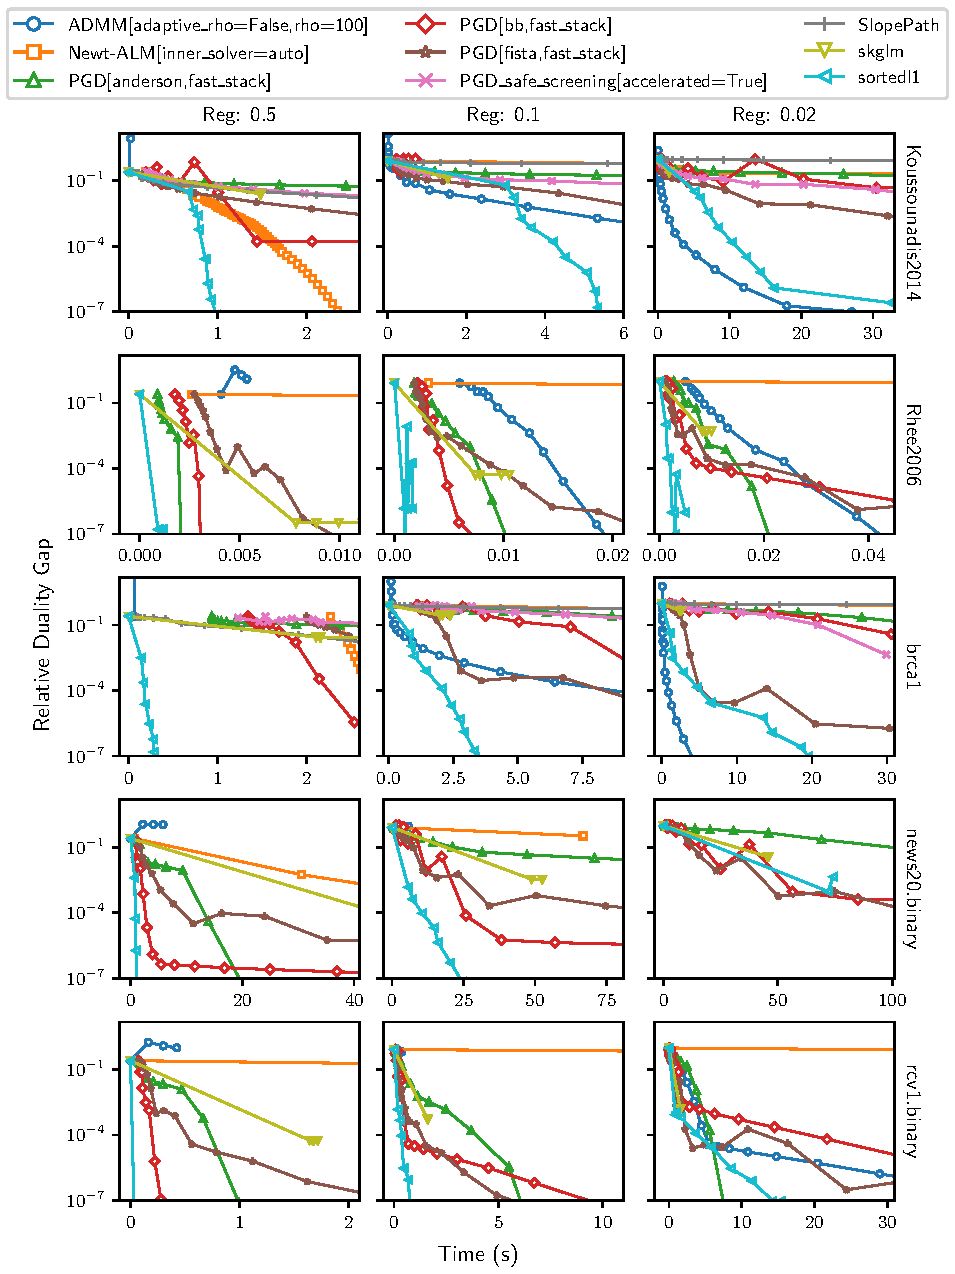
\includegraphics[width=\natwidth]{images/benchmark_single_real.pdf}
  \caption{%
    Performance of the solvers for the single solution benchmark for five
    different real data sets~(\autoref{tab:real-data}) and three levels of
    regularization. Please see the text for information about the data and
    setup of the experiment.
  }
  \label{fig:real-data-single}
\end{figure}

\subsection{Path}\label{sec:path-benchmark}

Here, we present benchmarks
on a subset of the real data sets from \autoref{tab:real-data}. We parameterize
the benchmark using the length of the path, using 50, 100, and 200 steps. We
present the results as the maximum relative duality gap along the path.

The results are presented in \autoref{fig:real-data-path}. Note that the interpretation
of progress towards convergence does not hold quite the same way as for the single
solution benchmarks since we fit a full path. Nevertheless, we note that our
implementation is the fastest by a large margin.

\begin{figure}[tp]
  \centering
  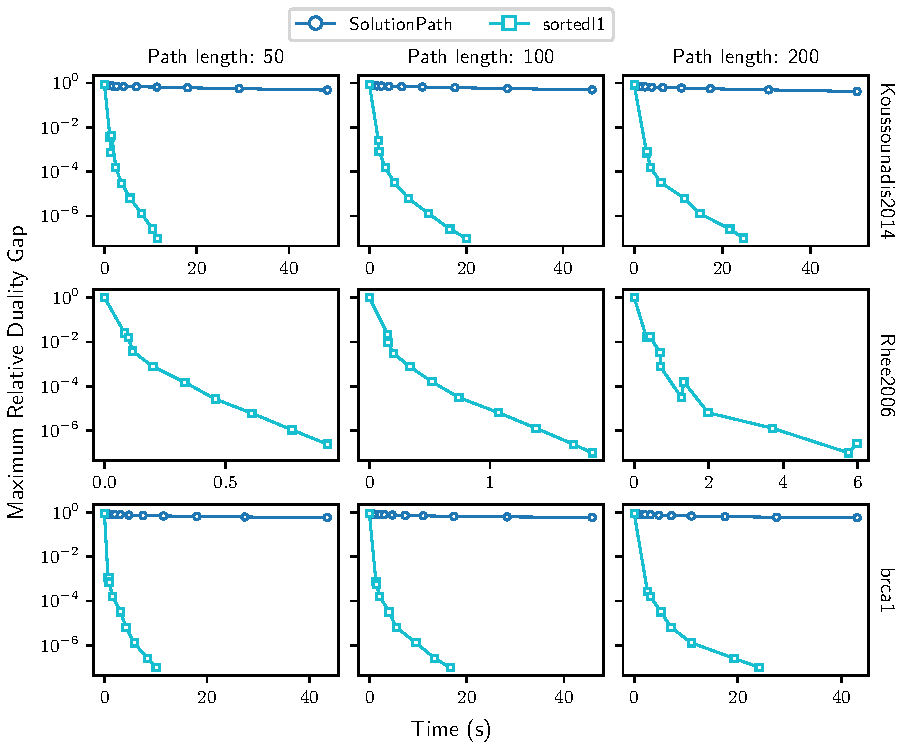
\includegraphics[width=\natwidth]{images/benchmark_path_real.pdf}
  \caption{%
    Benchmark for fitting the full regularization path on real data sets with
    varying path lengths. The plot show the maximum relative duality gap across all
    solutions along the regularization path.
  }
  \label{fig:real-data-path}
\end{figure}

Taken together, our benchmarks show that our method performs better
than all the competing methods.

\section{Application to real-world data}\label{sec:realdat}

To illustrate the practical utility of SLOPE, we applied it to a metabolomics
dataset from \citet{Godlewski2023}, comprising plasma measurements from glioma
patients and healthy controls. The dataset contains 165 samples (94 glioma
cases and 71 controls), each with 139 metabolite features.

We first create the design matrix \texttt{X} and the response vector
\texttt{Y}:

\begin{Code}
R> glioma_dat <- readRDS("./code/glioma_dat.RDS")
R> X <- scale(glioma_dat[, -1])
R> Y <- glioma_dat[, 1][[1]]
\end{Code}

We then fit a SLOPE model with cross-validation to select the regularization
parameter. The function \texttt{cvSLOPE()} performs $K$-fold cross-validation
and optimizes over~$\alpha$:

\begin{Code}
R> slope_cv <- cvSLOPE(X, Y, q = 0.1, family = "binomial", measure = "auc")
R> alpha_cv <- slope_cv$optima$alpha
R> slope_model <- SLOPE(X, Y, q = 0.1, family = "binomial", alpha = alpha_cv)
\end{Code}

Predicted probabilities for new data can be obtained with the \texttt{predict()}
method:

\begin{Code}
R> pred_prob <- predict(slope_model, X, type = "response")
\end{Code}

For illustration, we also split the data into training and test sets. This
allows us to evaluate out-of-sample classification performance when
distinguishing glioma patients from healthy controls:

\begin{Code}
R> set.seed(222)
R> train_index <- caret::createDataPartition(Y, p = 0.7, list = FALSE)
R> X_train <- X[train_index, ]
R> Y_train <- Y[train_index]
R> X_test  <- X[-train_index, ]
R> Y_test  <- Y[-train_index]
\end{Code}

In this example, SLOPE achieved an AUC of 0.978 on the test set, while the lasso
obtained 0.94. More importantly, SLOPE selected a richer set of features (25
metabolites grouped into 10 clusters), compared to 10 variables selected by the
lasso. One of the unique features of the R implementation is the ability to
visualize the clustering of coefficients with the \texttt{plotClusters()}
function\footnote{This functionality is specific to the R package.}. The plot
highlights groups of variables with coefficients of the same magnitude (up to
sign):

\begin{Code}
R> fit_pat <- SLOPE(X, Y, q = 0.1, pattern = TRUE, family = "binomial")
R> SLOPE::plotClusters(fit_pat, include_zeroes = FALSE)
\end{Code}

\begin{figure}[tp]
  \centering
  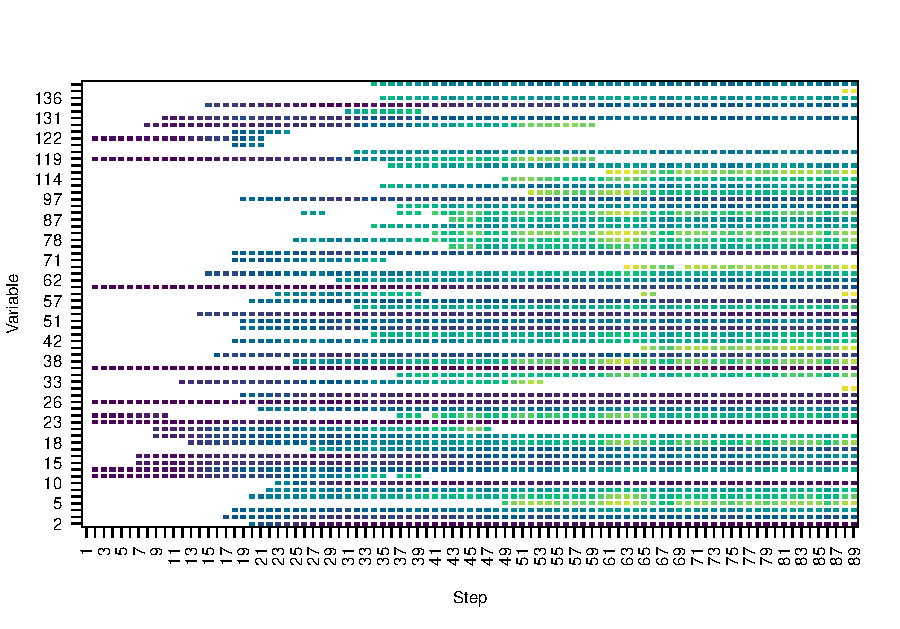
\includegraphics[width=\textwidth]{images/glioma-clusters.pdf}
  \caption{Cluster structure of metabolites selected by SLOPE. Variables are
  grouped by effect size, with colors indicating distinct clusters.}
  \label{fig:real-data-clusters}
\end{figure}

This produces a cluster map of selected metabolites, revealing biologically
meaningful groupings. For example, both SLOPE and the lasso consistently
identified \textit{kynurenine}, a known glioma biomarker \citep{du2020both}. SLOPE additionally
highlighted \textit{tryptophan} and several carnitine derivatives (e.g.,
acetylcarnitine and propionylcarnitine), which have recently been proposed as
glioma biomarkers \citep{wang2024genomic}. Other significant amino acids such as
\textit{phenylalanine} and \textit{lysine} \citep{koslinski2023comparative, srivastava2025amino} were selected by both SLOPE and lasso.
.

Overall, this example demonstrates how the package can be applied in practice.
Beyond predictive performance, its functionality, such as cross-validation,
prediction, and clustering visualization makes it a useful tool for
high-dimensional biomedical data analysis, where interpretability and feature
selection are central.

\section{Discussion}\label{sec:discussion}

SLOPE is an appealing model for high-dimensional regression problems that is
able to recover sparsity and ordering patterns in the solution, which sets it
apart from similar models such as the lasso and elastic net. Unlike these models
however, SLOPE represents a more challenging optimization problem due to the
penalty term's inseperability.

Despite the complexity of the problem, we have here presented a collection of
packages (in \proglang{R}, \proglang{Python}, and \proglang{Julia}) that offer
efficient and feature-rich implementations of SLOPE. We hope that this
endeavour will make SLOPE accessible to a wider audience and note that ours are
the first packages that implement SLOPE in these languages. At the time of
writing, the only other implementation of SLOPE is \pkg{skglm}, which is
available in \proglang{Python}. For \proglang{R} and \proglang{Julia}, ours are
the only available implementations.

We have shown that the performance of our software is unparalleled
compared to other algorithms and implementations, both for fitting
the full regularization path as well as for single solution, and
have shown these in a series of benchmarks on both real and simulated
data.

Our results are similar to those of \citet{larsson2023}, which features the
same algorithm, except that the current implementation fares better. We
believe this is likely due to the addition of screening rules and improvements
to the algorithm and implementation. One difference from \citet{larsson2023} is
the performance of the Newt-ALM method, which in the current benchmarks have
performed better. We have made improvements to the algorithm here that we think may
help explain this fact.

\citet{dupuis2024} benchmarked the Python implementation of the hybrid
algorithm from \citet{larsson2023} (that our algorithm is based on) against
their approximate homotopy method and showed that their method performed better
in one case and worse in another. In our benchmarks, however, we have
consistently found our algorithm to be superior. One reason for this is that
\citet{dupuis2024} used a stringent stopping criterion\footnote{A duality
  gap of \(10^{-10}\).} for their benchmarks. Another is that the problem sizes in
our benchmarks are generally larger. A third is, again, that our implementation
is improved compared to \citet{larsson2023}.

Although our packages are full-fledged implementations of SLOPE, there are
still some features that are missing. For instance, we do not yet support
observation weights or the full suite of loss functions from the family of
generalized linear models. We also do not yet support the group sorted \(\ell_1\)
norm, which would allow an alternative penalization scheme for multivariate
response problems. In addition, several possible improvements to the hybrid
method could be considered, such as accelerated and parallelized coordinate
steps. We leave these possibilities to future work but want to stress that our
packages are modular and have been designed with extensibility in mind, which
we hope will facilitate the addition of new features in the future. Because all
of the packages rely on the same \proglang{C++} library, contributions will
also propagate directly to the higher-level packages in \proglang{R},
\proglang{Julia}, and \proglang{Python}.

We hope that our packages will be useful for researchers and practitioners
alike and that the design of our software suite might inspire others to more
closely couple the available features of \proglang{R}, \proglang{Python}, and
\proglang{Julia} and avoid redundant implementations of the same algorithms in
each language.

\bibliography{main}

\newpage

\begin{appendix}

  \section{Duality gap and convergence criteria}
  \label{sec:convergence-criteria-details}

  In detail, we transform the primal problem \(P\), defined in \autoref{eq:slope}, into a
  constrained problem, taking \(\alpha = 1\) without loss of generality:
  \begin{equation}
    % \label{eq:slope-constrained}
    \begin{aligned}
       & \minimize_{\beta_0 \in \mathbb{R},\beta \in \mathbb{R}^p} &  & \frac{1}{n} \sum_{i=1}^n f(x_i^\intercal \beta + \beta_0, y_i) + J_{\lambda}(\beta) \\
      % & \text{subject to}                                              &  & r_i = \link(\bm{x}_i^\intercal \bm{\beta}) - y_i, \quad i = 1, \ldots, n                                            \\
       & \text{subject to}                                         &  & r_i = \ilink(\beta_0 + x_i^\intercal \beta) - y_i, \quad i = 1, \ldots, n           \\
    \end{aligned}
  \end{equation}

  Since \(\beta_0 + x_i^\intercal \beta = g(r_i + y_i)\), we can write the Lagrangian as
  \[
    L(\beta_0,\beta,r,\delta) = \frac{1}{n} \sum_{i=1}^n f\big(g(r_i + y_i), y_i\big) + J_{\lambda}(\beta) - \sum_{i=1}^n \delta_i \left(g(r_i + y_i) - x_i^\intercal \beta - \beta_0 \right).
  \]
  This allows us to write the dual problem as
  \[
    D(\delta)  = \inf_r\left( \frac{1}{n} \sum_{i=1}^n f\left(g(r_i+y_i), y_i\right) - \delta_i g(r_i+ y_i)\right)
    % & \phantom{={}} + \inf_\beta \left(J_\lambda(\beta) - \delta^\intercal X\beta\right)   \\
    % & \phantom{={}} + \inf_{\beta_0} \left( -\delta^\intercal \bm{1} \beta_0\right)        \\
    - \sup_\beta \big((-X^\intercal \delta)^\intercal \beta -  J_\lambda(\beta) \big)
    - \sup_{\beta_0} \left( \delta^\intercal \bm{1} \beta_0\right).
  \]
  Here, we begin by noting that the infimum is attained at the point where
  \(r = \delta\)~\citep{fercoq2015}, which means that the value is
  \[
    \frac{1}{n} \sum_{i=1}^n f\left(g(\delta_i+y_i), y_i\right) - \delta_i g(\delta_i + y_i)
  \]
  in general, although loss-specific simplifications can be made. For instance, in the case of
  quadratic loss the expression evaluates to \(\frac{1}{2} \lVert y \rVert_2^2 - \frac{1}{2} \lVert \delta + y \lVert^2_2 \).

  Next, we observe that \(\sup_\beta \big((-X^\intercal
  \delta)^\intercal \beta -  J_\lambda(\beta) \big)\) is the Fenchel conjugate of
  the sorted \(\ell_1\) norm, which is the indicator function of the sorted
  \(\ell_1\) dual norm unit ball. Its value is
  \[
    \sup_\beta \big(z^\intercal \beta -  J_\lambda(\beta) \big) =
    \begin{cases}
      0      & \text{if } J^*_\lambda(z) \leq 1, \\
      \infty & \text{otherwise},
    \end{cases}
  \]
  where \(J^*_\lambda(z)\) is the sorted \(\ell_1\) dual norm, defined as~\citep{negrinho2014}
  \begin{equation}
    J^*_\lambda(z) = \max_{j=1,2,\dots,p}\left\{ \frac{\sum_{k=1}^j|z_{(k)}|}{\sum_{k=1}^j\lambda_k}\right\}
  \end{equation}

  Next, observe that \(\sup_{\beta_0} (\delta^\intercal \bm{1} \beta_0) = \infty\) unless
  \(\delta^\intercal \bm{1} = 0\).

  Taken together, this means that we have the following dual function:
  \begin{equation}
    D(\delta) = \begin{cases}
      \frac{1}{n} \sum_{i=1}^n f\left(g(\delta_i+y_i), y_i\right) - \delta_i g(\delta_i+ y_i) & \text{if } J^*_\lambda(-X^\intercal \delta) \leq 1 \text{ and } \delta^\intercal \bm{1} = 0 \\
      -\infty,                                                                                & \text{otherwise}.
    \end{cases}
  \end{equation}

  A natural dual point candidate for this problem is to pick
  \(\delta = r\), since
  at the optimum we have
  \[
    \bm{0} \in X^\intercal r + \partial J_\lambda(X^\intercal r)
  \]
  and, in addition require that the signs between agree.
  % TODO: Hand-wavy, clean up later.

  % To obtain a feasible dual point for this problem, we can use the
  % following fact about the stationarity condition of the primal problem,
  % namely that
  % \[
  %   \sum_{j=1}^k | g_{(j)} | \leq \sum_{j=1}^k \lambda_j |\beta_{(j)}| \quad \forall\; k = 1,2,\dots,p.
  % \]
  % where  \(g_j = x_j^\intercal r\) is the \(j\)th component of the gradient of loss function
  % with respect to \(\beta_j\)
  % and \(r\) the generalized residual, for which \(r_i = \ilink(x_i^\intercal \beta + \beta_0) - y_i\).

  To be a feasible point, however, we first center the point by its mean and
  scale it:
  \[
    \delta_j = \frac{r_i - \bar{r}}{\max\left\{1, J_\lambda^*\left(X^\intercal(r - \bar{r})\right) \right\}}
  \]
  which guarantees feasibility. We then obtain the following duality gap:
  \[
    P(\beta_0, \beta) - D(\delta).
  \]
  As a stopping criterion for the algorithm, we use the relative duality gap
  \[
    P(\beta_0, \beta) - D(\delta) \leq \varepsilon P(\beta_0),
  \]
  where \(\varepsilon >0\) is the user-defined tolerance level.
  The duality gap provides an upper bound on suboptimality for the problem, independent
  of solver and conditioning of the problem, which is not the case of
  convergence criteria based on changes in objective, gradients, or coefficients.

  The availability of the duality gap would also allow us to employ
  duality-gap based safe screening rules~\citep{fercoq2015} and
  working set strategies derived from these~\citep{massias2018}, which
  could furthermore be used to enhance our strategy with look-ahead
  screening rules~\citep{larsson2021a}. However,
  as noted in \citet{larsson2022d}, the marginal improvement
  of using duality-based screening strategies is minor, so we have
  opted not to implement these in our packages.

  \section{Solver details}\label{sec:solver-details}

  \begin{description}
    \item[sortedl1] The python package of our implementation of the hybrid
          proximal gradient/coordinate descent algorithm described in this work and
          \citet{larsson2023}. We use the randomized version of the coordinate descent
          updates.
    \item[Anderson PGD] The proximal gradient descent (PGD) algorithm with Anderson acceleration, which is a
          method for accelerating the convergence of fixed-point
          iterations~\citep{anderson1965,zhang2020}.
    \item[BB PGD] PGD with Barizilai--Borwein~\citep{barzilai1988} step sizes.

    \item[FISTA] The fast iterative shrinking and thresholding
          algorithm~\citep{beck2009}, which is an accelerated version of iterative
          soft-thresholding algorihthm (ISTA)~\citep{wright2009}.

    \item[Safe PGD] FISTA with acceleration using safe screening
          rules~\citep{elvira2023}.

    \item[ADMM] The alternating direction method of
          multipliers~\citep{glowinski1975,boyd2010}, which is a popular algorithm
          for solving convex optimization problems with constraints. In our experiments,
          we have used \(\rho = 100\) as a step size based on the
          results from \citet{larsson2023}.
          We considered using the heuristic \(\rho\) selection method from
          \citet{boyd2010}, but have avoided to do so since it, as shown by \citet{larsson2023},
          may lead to erratic convergence behavior in practice. We use \fct{lsqr}
          from \pkg{SciPy}~\citep{virtanen2020} to solve the linear system if
          \(\min\{n, p\} > \num{1000}\) and otherwise use solve the linear system
          as suggested by \citet{boyd2010}.

    \item[Newt-ALM] A semi-smooth Newton-based method~\citep{luo2019}. Our
          implementation of this method is based on that from \citet{larsson2023},
          but improved with better heuristics for selecting the inner solver,
          improved conjugate gradient solver, and
          a bug fix for the Woodbury-based solver. For the conjugate gradient solver,
          we use \fct{cg} from \pkg{SciPy}~\citep{virtanen2020}.

    \item[skglm] Another implementation of FISTA from the
          \pkg{skglm} package~\citep{bertrand2022}.

    \item[SolutionPath] An approximate homotopy method by \citet{dupuis2024},
          which is similar to the lars algorithm for the lasso~\citep{efron2004}.
  \end{description}

\end{appendix}

\end{document}
